% D.5 等腰△ABC（AB=AC），D∈AB、E∈AC，BD=CE，BE、CD 交于 P
\documentclass[tikz,border=4pt]{standalone}
\usepackage{ctex}
\usepackage{amsmath}
\usetikzlibrary{calc, decorations.markings}
\begin{document}
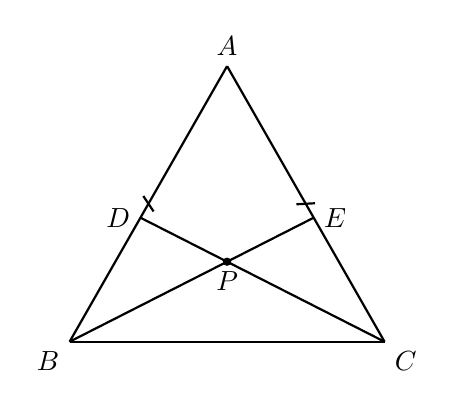
\begin{tikzpicture}[scale=1.0, thick,
  tick/.style={postaction={decorate, decoration={markings,
    mark=at position 0.5 with {\draw (-1.5pt,-3pt) -- (1.5pt,3pt);}}}}]
  \coordinate (A) at (0, 3.5);
  \coordinate (B) at (-2, 0);
  \coordinate (C) at (2, 0);
  \coordinate (D) at ($(A)!0.55!(B)$);
  \coordinate (E) at ($(A)!0.55!(C)$);
  % P 是 BE 与 CD 的交点（手工计算交点）
  \coordinate (P) at (intersection of B--E and C--D);

  \draw[tick] (A) -- (B);
  \draw[tick] (A) -- (C);
  \draw (B) -- (C);
  \draw (B) -- (E);
  \draw (C) -- (D);

  \node[above]       at (A) {$A$};
  \node[below left]  at (B) {$B$};
  \node[below right] at (C) {$C$};
  \node[left]        at (D) {$D$};
  \node[right]       at (E) {$E$};
  \node[below]       at (P) {$P$};
  \fill (P) circle (1.5pt);
\end{tikzpicture}
\end{document}
